\documentclass[t]{beamer}
\usetheme{Rochester}
\usecolortheme{beaver}
\usepackage{graphicx}
\usepackage{geometry}

\title{MinusMinusEnergy}
\subtitle{Energy Switzerland Challenge}
\author
{M.\,Busenhart \and M.\,Winkler \and M-L.\,Achart \\\and P.\,Wiese \and Y.\,Niedermayr}
\date[BETH 2019]
{BETH - Blockchain for Sustainability, 2019}
\subject{Computer Science}

\logo{ \begin{minipage}{10.2cm}
\includegraphics[height=1.5cm]{BETH.png}\end{minipage} \begin{minipage}{2.5cm}
\includegraphics[height=1.2cm]{swissenergy.png}\end{minipage}}

\begin{document}
  \frame{
    \titlepage
  }
  \begin{frame}
    \frametitle{Concept}
    \begin{figure}
    	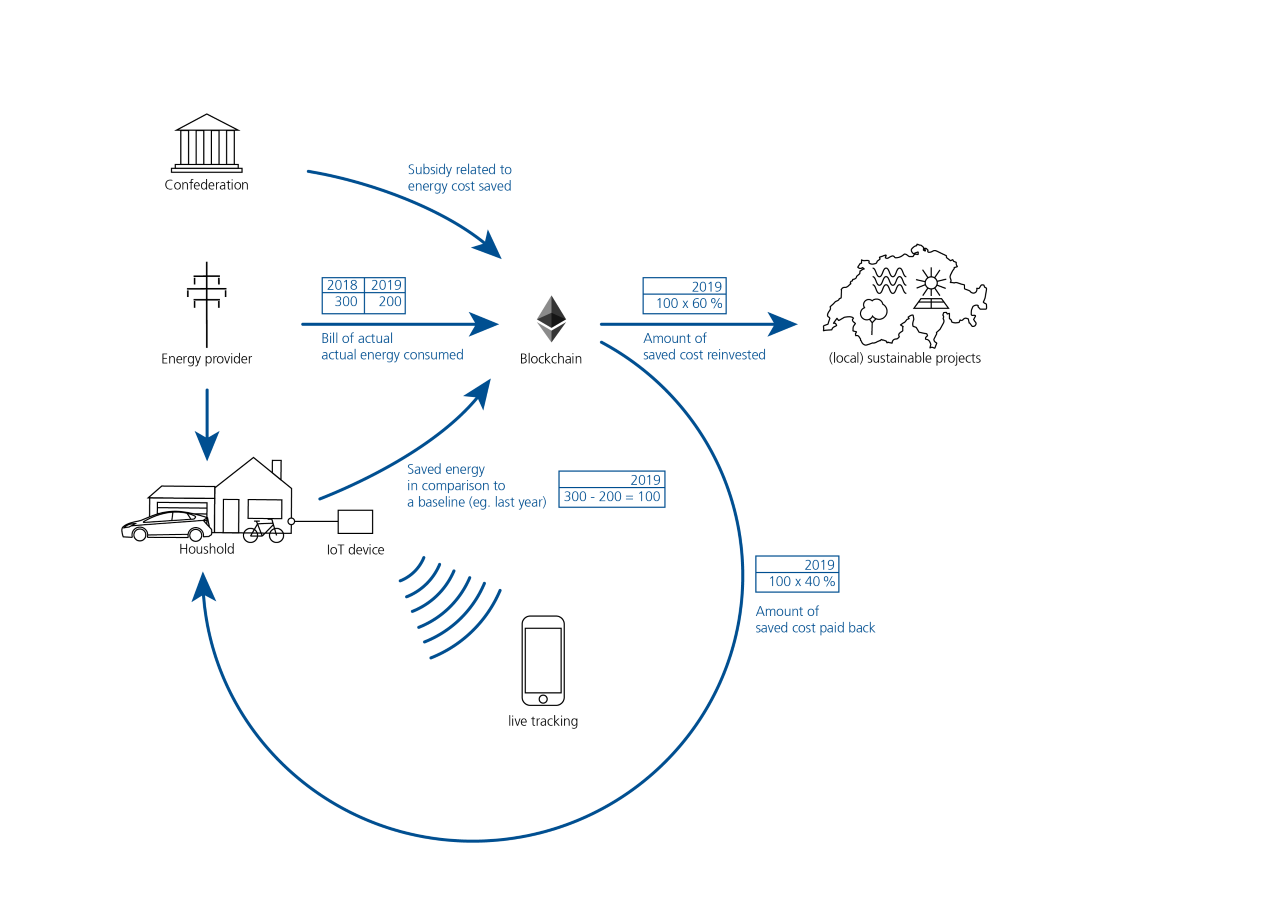
\includegraphics[width=1\linewidth]{concept.png}
    \end{figure}
  \end{frame}

  \begin{frame}
		\frametitle{Current Implementation}
		\begin{figure}
			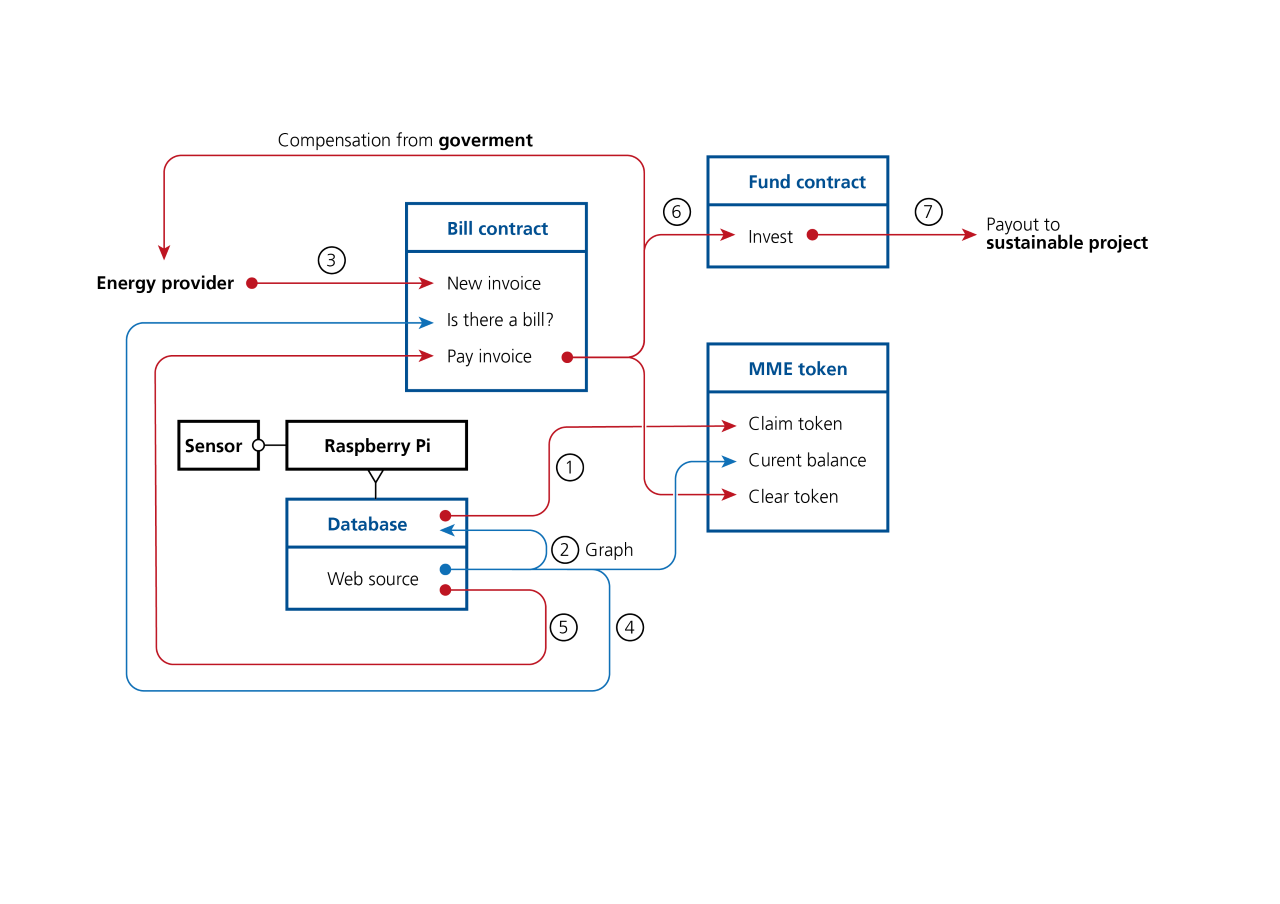
\includegraphics[width=1.1\linewidth]{implementation.png}
		\end{figure}
  \end{frame}

  \begin{frame}[t]
    \frametitle{Disruptive Potential and Further Development}
    \begin{itemize}
    	\item{Simplified/automated billing thanks to smart contracts.}
    	\item{Data standardisation with smart metering.}
    	\item{Secured data transmission and storage on the Blockchain.}
    	\item{IoT devices to monitor energy consumption.}
		\item{Reward system fully involving the consumer.}    
		\item{Relevant visualization and live tracking as incentive.}
		\item{Consumer gains power and controls the amount and destination of reinvested saved cost.}
		\item{New paradigm: when the consumer saves energy, he does not only pay less, he also earns more.}
		\item{Could be a first step toward decentralized energy grid.}
    \end{itemize}
    \end{frame}

  \begin{frame}
    \frametitle{Demo}
    content: insert gif
  \end{frame}
\end{document}
